\begin{figure}[h!]
	\centering
	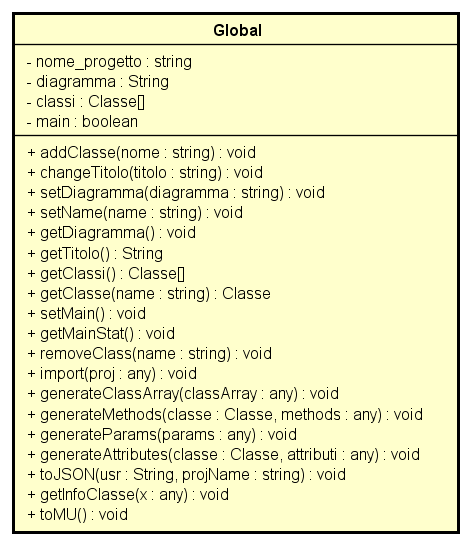
\includegraphics[scale=0.8]{res/sections/SpecificaFrontEnd/Services/Disegnetti/global.png}
	\caption{Diagramma della classe Global}
\end{figure}

\begin{itemize}
	\item \textbf{Descrizione:}\\
	
	\item \textbf{Utilizzo:}\\
	
	\item \textbf{Attributi:}
		\begin{itemize}
			\item \emph{-nome\_progetto: string}\\
			Memorizza il nome del progetto
			\item \emph{-diagramma: string}\\
			Memorizza il diagramma
			\item \emph{-classi: Classe[]}\\
			Memorizza le classi dell'array
			\item \emph{-main: boolean}\\
			True se il metodo main presente
		\end{itemize}
	\item \textbf{Metodi:}
		\begin{itemize}
			\item \emph{+addClasse(nome: string)}\\
    		Crea una nuova classe\\
    		\textbf{Parametri:}
    		\begin{itemize}
    			\item \emph{nome: string}\\
    			Nome della classe
    		\end{itemize}
    		\item \emph{+changeTitolo(titolo: string)}\\
    		Modifica il nome del progetto\\
    		\textbf{Parametri:}
    		\begin{itemize}
    			\item \emph{titolo: string}\\
    			Nome del progetto
    		\end{itemize}
    		\item \emph{+setDiagramma(diagramma: string)}\\
    		Resetta il diagramma\\
    		\textbf{Parametri:}
    		\begin{itemize}
    			\item \emph{diagramma: string}\\
    			Diagramma da resettare
    		\end{itemize}
    		\item \emph{+setName(name: string)}\\
    		Modifica il nome della classe selezionata\\
    		\textbf{Parametri:}
    		\begin{itemize}
    			\item \emph{name: string}\\
    			Nuovo nome della classe
    		\end{itemize}
    		\item \emph{+getDiagramma()}\\
    		Ritorna la stringa diagramma
    		\item \emph{+getTitolo()}\\
    		Ritorna il nome del progetto
    		\item \emph{+getClassi()}\\
    		Ritorna l'array delle classi
    		\item \emph{+getClasse(name: string)}\\
    		Ritorna la classe\\
    		\textbf{Parametri:}
    		\begin{itemize}
    			\item \emph{name: string}\\
    			Nome della classe da ritornare
    		\end{itemize}
    		\item \emph{+setMain()}\\
    		Setta a true l'attributo main
    		\item \emph{+getMainStat()}\\
    		Ritorna il valore dell'attributo main
    		\item \emph{+removeClass(name: string)}\\
    		Rimuove una classe dall'array\\
    		\textbf{Parametri:}
    		\begin{itemize}
    			\item \emph{name: string}\\
    			Nome della classe da rimuovere
    		\end{itemize}
    		\item \emph{+import(proj: any)}\\
    		Importa il progetto\\
    		\textbf{Parametri:}
    		\begin{itemize}
    			\item \emph{proj: any}\\
    			Progetto da importare
    		\end{itemize}
    		\item \emph{+generateClassArray(classArray: any)}\\
    		Genera la stringa con le informazioni della classe\\
    		\textbf{Parametri:}
    		\begin{itemize}
    			\item \emph{classArray: any}\\
    			Array della classe
    		\end{itemize}
    		\item \emph{+generateMethods(classe: Classe, methods: any)}\\
    		Genera la stringa dei metodi\\
    		\textbf{Parametri:}
    		\begin{itemize}
    			\item \emph{classe: Classe}\\
    			Classe di cui generare i metodi
    			\item \emph{methods: any}\\
    			Metodo
    		\end{itemize}
    		\item \emph{+generateParams(params: any)}\\
    		Genera la stringa dei parametri\\
    		\textbf{Parametri:}
    		\begin{itemize}
    			\item \emph{params: any}\\
    			Lista dei parametri
    		\end{itemize}
    		\item \emph{+generateAttributes(classe: Classe, attributi: any)}\\
    		Genera la stringa degli attributi\\
    		\textbf{Parametri:}
    		\begin{itemize}
    			\item \emph{classe: Classe}\\
    			Classe
    			\item \emph{attributi: any}\\
    			Lista di attributi
    		\end{itemize}
    		\item \emph{+toJSON(usr: String, projName: string)}\\
    		Trasforma il progetto in un file JSON\\
    		\textbf{Parametri:}
    		\begin{itemize}
    			\item \emph{usr: String}\\
    			Username dell'utente
    			\item \emph{projName: string}\\
    			Nome del progetto
    		\end{itemize}
    		\item \emph{+getInfoClasse(x: any)}\\
    		Ritorna tutte le informazioni della classe\\
    		\textbf{Parametri:}
    		\begin{itemize}
    			\item \emph{x: any}\\
    			Classe
    		\end{itemize}
    		\item \emph{+toMU()}\\
    		Aiuta a trasformare il progetto in un JSON
		\end{itemize}
\end{itemize}